% !TEX root = ./../main.tex
\chapter{Empirical Force--Field model}
\label{chap:EmpiricalFF}
As we have seen in the previous section \ac{MD} provides a variety of tools for solving the time evolution of a
$N$--particle system. Due to the possibility to capture different length and time scales \ac{MD} simulations can
be used in a variety of systems, such as set of atoms, molecules or more complex system such as protein and
macromolecules systems. In each of these systems, depending on the \textit{interaction model} and its
\textit{parametrization}, we will be able to describe crucial molecular--level processes, such as hydrogen bond
formation in organic molecules, which happen on the picoseconds time scale; or study slow processes such as the
diffusion of massive colloidal particles, taking place on time scales of milliseconds if not seconds. Considering soft or condensed mater, the most relevant for this thesis, the main processes of interest
ranging from protein folding to glass transitions, from surface diffusion to ligand--receptor binding take place
on longer time scales (several ns) and involve a larger number of atoms ($N \gg 10^4$).

Hence with soft or condensed matter systems, in order to remove some \ac{DOF} due to the necessity to increase
the time step and speed up the simulation, a crucial role is played by the \textit{Born--Oppenheimer
approximation}. It says that we can separate the motion of the electrons by the motion of the atomic nuclei. This
is done in order to integrate out the high frequency electrons' motions. If, for some particular system, we want
to know precisely the dynamics of the electrons we have to introduce quantum mechanical methods that are, even
for a small number of particles ($N\sim 10^2$), very computationally time consuming. In the following, when we
speak about atoms or chemical moieties we refer to it as for nuclei coordinates only without considering
electrons at all.

Nevertheless atom or molecule interactions, such as bond formation, are mediated by the electron interactions.
Thus, to describe the dynamics of such a system with a classical \ac{MD} tools and the Born--Oppenheimer
approximation, it is necessary to develop an \textit{empirical model of the inter--atom interactions} that mimics
the interactions behavior. Since forces are derived from the \ac{PEF}, a typical choice, when it is possible, for
example with organic systems, is to model the inter--particle interactions by a set of pairwise addictive
potentials that avoid any many--body calculations. Nevertheless for some systems this is impracticable, for
example, for metal cores we need to consider the many--body calculations or an effective many--body potential
that take into account the behavior of all metal atoms in the core. A typical solution is to use the many--body
potential developed by Gupta (see \cite{Leach} for more details about metals treatment at \ac{MD} level). The set
of functional forms of the inter--particle interaction potentials and its parameterization are collected into the
so called empirical \acf{FF}. The meaning of \textit{empirical} is that most of the functional forms of the
interactions has no ``first principle'' justification: they are chosen as a compromise between accuracy and
computational efficiency.
%Further it is necessary to stress out that a \ac{FF} is a well defined single entity containing the simulation parameters, the functional models of the interactions and also its parameterizations (and the way to obtain it). All the parameters of a \ac{FF} are in harmony to each other thus changing some parameters without retesting whole \ac{FF} is not allowed because, maybe, one can destroy the whole \ac{FF}.

For biomolecular applications two main classes of \acp{FF} exist: the \textit{atomistic} \acp{FF} in which basic
particles are atoms, and the \textit{\ac{CG}} \acp{FF} in which the basic particles represent atom groups or
small chemical moieties. In this case, even the way to realize the grouping, called \textit{mapping}, is part of
the \ac{FF} itself. Different \ac{CG} \acp{FF} can use different mapping methods even with the same functional forms.

In the following we will add some other information about \acp{FF} and describe the principal functional forms
for modeling the inter--particle interactions and how to treat them in an \ac{MD} simulation. While in the next
section we will focus on the main \ac{CG} \ac{FF} used in this thesis work: the \textacr{MARTINI} \ac{FF}
developed by Marrink \etal\, \cite{Martini}.

\paragraph{\textbf{\textacr{parameterization}}} In general the functional forms for potential interactions are
common to all particles in the system. The \ac{FF} is completed by a set of empirical parameters that
characterize the interaction between different types of particles, whether they are atoms or whole chemical
groups. Interaction parameters are empirical in the sense that they are assigned to reproduce a small set of
target properties on a small group of systems. These target properties can be derived from experimental
measurements or from finer--level calculations or simulations. Nowadays, atomistic and \ac{CG} biomolecular
\acp{FF} come as ``packages'' of parameters and functional forms appropriate for the description of a large
variety of chemical compounds in the liquid and solid phases.

\paragraph{\textbf{\textacr{transferability}}} As described above the parameterization of a \ac{FF} involves a
small set of test systems for which some set of target proprieties are reproduced. The main characteristic of a
\ac{FF} is the \textit{transferability} that means the ability of the model to describe different situations that
differ from those used at the parameterization stage. Of course one would expect to be able to make some
predictions for a bigger variety of systems and for other proprieties not used in the parametrization stage.
Common faults of organic \acp{FF} concern, for example, phase transitions of organic compounds and phase
transition temperatures.

\section{Inter--particle interactions}
For biomolecular applications the inter--particle interaction potentials are divided into two main classes: the
\textit{bonded interactions} involving particles within the same molecules and the \textit{non--bonded
interactions} engaging all particles in the system and which usually represent the Van der Waals and the
electrostatic interactions. In the following the most common and general functional form for the \ac{PEF} is
descried. In general the \ac{PEF} can be always splitted in a bonded and non--bonded contributions:
\begin{equation*}
	U(\vec r) = U_{\text{b}}(\vec r) + U_\text{nb}(\vec r)
	\label{eq:FFPEF}
\end{equation*}

The bonded contribution is generally described by the following terms
\begin{equation}
	\begin{aligned}
	U_{\text{b}}(\vec r) = &\frac{1}{2}\sum_{\text{bonds}} \frac{1}{2}k_i^b(l_i - l_{i0})^2\ + \frac{1}{2}\sum_{\text{angles}} k_i^a (\theta_i - \theta_{i0})^2 +\\
		 	& +\frac{1}{2}\sum_{\text{torsions}} V_n(1+\cos (n\omega - \gamma))
	\end{aligned}
	\label{eq:bondPEF}
\end{equation}
the first two terms are harmonic potentials which model respectively the energy contribution due to the deviation
from reference bond length $l_{i0}$ and a bond angle $\theta_{i0}$. $k_{bi}$ and $k_{ia}$ are the bond and angle
elastic constants. The bond contribution involve a set of two particles in the some molecule while the angle
contribution a set of three particles in the same molecule. The last term in equation~\eqref{eq:bondPEF} concerns
the energy contribution due to the bond torsional change. It involves four particles in the same molecule and
mimic the energy barrier needed to rotate the bond angle along the bond axis. $\omega$ is the torsional angle,
$\gamma$ is a phase factor, $V_n$ qualitatively describes the energy barrier for each $n$--th components and $n$
is defined as the number of minima for each components.

The non--bonded contribution is described by the following terms
\begin{equation}
	U_\text{nb}(\vec r) = \sum_{i=1}^N \sum_{j>i} \left ( {4\epsilon_{ij} \left ( \left ( \frac{\sigma_{ij}}{r_{ij}} \right )^{12} - \left ( \frac{\sigma_{ij}}{r_{ij}} \right )^6 \right )  + \frac{q_iq_j}{4\pi\varepsilon_0 r_{ij}}} \right )
	\label{eq:nonbonPEF}
\end{equation}
The first term is the energy contribution due to the Van der Waals interactions modeled as a Lennard--Jones
$12-6$ potential, fully characterized by the constants $\sigma_{ij}$ and $\epsilon_{ij}$ proper for each
particles pair. The last term is the electrostatic energy contribution described by the particle charge $q$. The
non--bonded interactions involve obviously all particles in the system, but for particles belonging to same
molecule they are computed only if they are separated by at least three bonds, i.e. if their interactions are not
described by bonded terms. The various contributions described above are schematically represented in
figure~(\ref{fig:FFInteraction}).
\begin{figure}[!ht]
	\centering
	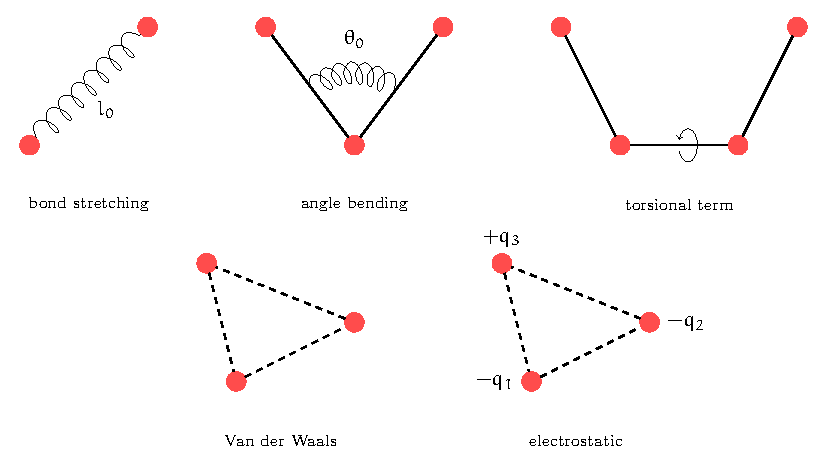
\includegraphics[width=0.8\textwidth]{./img/interPartInt/interPartInt}
	\caption{Schematic representation of the common inter--atom interactions for biomolecular applications: bond stretching, angle bending, torsional term, Van der Waals and electrostatic interactions.}
	\label{fig:FFInteraction}
\end{figure}

\subsection{Non--bonded interactions: general aspect}
%\label{sec:nonbonded}
The bonded interactions, as we can see in equation~\eqref{eq:bondPEF}, are at \textit{fixed range}, meaning that
they depend, for example, on the equilibrium bond length that is fixed. Moreover, usually in standard \ac{MD}
simulations the bond break is not taken into account. The non--bonded interactions, instead, are at non--fixed
range because they depend on the inter--particles distance $r_{ij}$ and decay to zero as a power of
$r_{ij}^{-d}$. Depending on the power order $d$ compared to the dimensionality $s$ of the system they are split
into \textit{short range} if $d>s$ and \textit{long range} interactions if $1 \le d < s$. For example, as we
shall see later, the Lennard--Jones $12-6$ potential decays to zero as $r^{-6}$ then it is a short range
interaction, while the electrostatic is a long range interaction since it decays to zero as $r$.

\subsection{Cut--off, shift and switch methods}
As we have mentioned in section~\ref{sec:neighbor} the calculations of non--bonded interaction energy
contributions is one of the most time consuming part of an \ac{MD} simulation. Even if we use a simple pairwise
additive potential their calculation scale as $\sim N^2$. Thus, especially for short range interactions, various
methods were developed in order to speed--up the simulation. The \textit{cut--off} method is the most used to
treat the short range interactions and, in some cases, even the long range ones. Taking one particle into
account, the general idea is to evaluate the non--bonded interactions with all other particles that are closer to
the first for a distance $r_c$, called \textit{cut--off} radius, otherwise the interactions is set to $0$. This
means that the new potential is of the form
\begin{equation*}
v^*(r) = \left \{
	\begin{aligned}
&v(r) & \quad & r \le r_c \\
&0    & \quad & r >   r_c
	\end{aligned} \right .
\end{equation*}

This generates a discontinuity in the potential and in its first derivatives, i.e. in the forces: this is bad for
energy conservation. A trick for solving the discontinuity of the potential and to improve the energy
conservation is to apply also a \textit{shift} of the potential value at $r_c$ so that $v^*(r_c) = 0$. Adding a
constant will not affect the force calculations. The potential becomes
\begin{equation*}
v^*(r) = \left \{
	\begin{aligned}
&v(r) - v(r_c) & \quad & r \le r_c \\
&0    & \quad  & r >   r_c
	\end{aligned} \right .
\end{equation*}

Moreover, to solve the discontinuity of the forces, that can cause some instability, a simple possibility is to
consider a linear term proportional to the first derivative of the potential, such as
\begin{equation*}
v^*(r) = \left \{
	\begin{aligned}
&v(r) - v(r_c) - \left . \frac{dv(r)}{dr}\right |_{r_c}\ (r - r_c) & \quad & r \le r_c \\
&0    & \quad  & r >   r_c
	\end{aligned} \right .
\end{equation*}
The shift methods can make the potential quite different from the original one. So this have to be properly taken
into account in order to retrieve the correct thermodynamics proprieties.

Another powerful method to solve the discontinuity problem of the potential and forces is the \textit{switch}
method. The general idea is to consider two cut--off radii  $r_{c1}$ and $r_{c2}$. If $r \le r_{c1}$ the original
form is used; while if $r > r_{c2}$ the potential is set to zero. If $r_{c1} < r \le r_{c2}$ a \textit{switching
function} is considered in order to \textit{smoothly} switch the potential to zero.

It is important to stress out that even the method used to treat the interactions, as the cut--off radii and
eventually the switching function, are part of the simulation parameters that are, in turn, part of the \ac{FF}.
So they are interdependent with the model parameterization, and should never be changed without retesting the
target properties of the parameterization.

\section{Van der Waals interactions}
Van der Waals forces are a set of interactions that can be ascribed to quantum dynamic effects. In general they
are described by a sum of a repulsive and an attracting term. The former effectually takes into account the Pauli
exclusion principle between electron clouds; the latter is related to the dipole--dipole interactions (Keesom
forces), dipole--induce dipole interactions (Debye forces), induced dipole--induced dipole interactions, London
dispersion forces, hydrogen bonding and entropy effects, that involves both polar and non--polar atoms.

The usual way to treat the Van der Waals interactions is to use a pairwise Lennard--Jones potential. The most
common exponents for the attractive and repulsive contributions are $6$ and $12$, respectively. The former has
physical meaning: calculating the repulsive part of the Van der Waals interaction for a simple system in a
semi--classical approximation gives a potential energy contribution that vanishes as $r^{-6}$. While the latter
is only for computational reason: giving the $r^{-6}$ term it is efficiency to calculate $r^{-12}$ as the square
of $r^{-6}$. Thus it is just a common choice and other exponents can do the job, depending on the system in
study. The general form for a $12-6$ Lennard--Jones potential is the following
\begin{equation}
	v(r) = 4\epsilon\left ( \left ( \frac{\sigma}{r}\right )^{12}  - \left ( \frac{\sigma}{r} \right )^6 \right ) = \frac{C_{12}}{r^{12}} - \frac{C_{6}}{r^{6}}
	\label{eq:lj126}
\end{equation}
where $C_{12} = 4\epsilon\sigma^{12}$, $C_{6} = 4\epsilon\sigma^{6}$ and $r$ is the pairwise particles distance.
$\epsilon$ is related to the absolute value of minimum while $\sigma$ is related to the position of the minimum
of the potential: $r_{\text{min}} = 2^{\nicefrac{1}{6}}\sigma$, often referred to by Van der Waals radius. These
constants are proper for each particle pair. The attractive contribution is due to the negative part proportional
to $r^{-6}$ while the repulsive one is due to the positive part proportional to $r^{-12}$. In
figure~(\ref{fig:LG12511}) a plot of the function~\eqref{eq:lj126} with $\epsilon = \sigma = 1$ is shown.
\begin{figure}[!ht]
\centering
	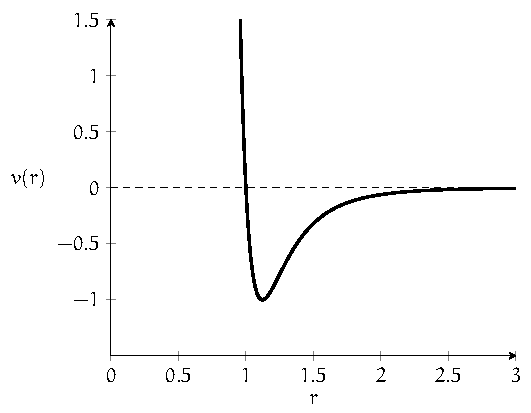
\includegraphics[width=0.6\textwidth]{./img/LJ126/LJ126}
	\caption{Plot of a Lennard--Jones interaction potential with $\epsilon = \sigma = 1$.}
	\label{fig:LG12511}
\end{figure}

The simplest and computationally most efficient way to treat a Lennard--Jones function, and in general all the
short range interactions, is to use the cut--off method together with the shift or switch methods in order to
obtain a continuous potential and/or a continuous forces. As we can see from figure~(\ref{fig:LG12511}) the
Lennard--Jones potential vanishes rapidly with distance: at $r \sim 2\sigma$ its value is less then $1\%$ of the
value in $r \sim \sigma$. A good choice for the cut--off is then of the order of $r_c \sim 2\sigma \div 3\sigma$.

\section{Electrostatic interactions}
\label{sec:electrostaticInt}
Despite the long range characteristic of the electrostatic interaction, for computational efficient reason, most
of the \acp{FF} for biomolecular applications treat them in the same way as a short range interaction by a
cut--off method\footnote{In general, for computational reason, a common choice is to consider the same cut--off
for Van der Waals and electrostatic interactions.}. Of course this is an approximation and can lead to serious
issues in those proprieties or systems that strongly depend on the electrostatic interactions. As an example we
report some situations in which the use of the short--range electrostatics can lead to artifacts: they are
related to the development of a good polar solvent model (a good treatment of the electrostatic proprieties of
water is really important for biological applications), as well as to the study of the interactions of charged
particles with polar solvents, transport processes of charged moieties, calculations of the electrostatic
potential inside macromolecules and so on. The calculation of the electrostatic energy contribution requires to
take into account \textit{all particles} in a system, even all the periodic images due to the \ac{PBC}. This
leads to a loss of computational efficiency.

If we consider only the simulation box the electrostatic energy contribution is
\begin{equation}
	U = \frac{1}{2}\sum_{i=1}^N\sum_{j\ne i}^N\frac{1}{4\pi\varepsilon_0}\frac{q_iq_j}{r_{ij}}
	\label{eq:electrostatic}
\end{equation}
where $q_i$, $q_j$ and $r_{ij}$ are the charges and the distance, respectively, between particles $i$ and $j$.
But we need also all image boxes. Let us suppose, for simplicity, a cubic box of size $L$. We can
define a tern of integer numbers $(n_x,\ n_y,\ n_z)$, $n_i=0,1,2,\cdots$ so that the position of all other image
boxes, with respect to the central simulation box, is $\vec n = L (n_x,\ n_y,\ n_z)$. Then the energy
contribution becomes
\begin{equation}
	U = \frac{1}{2}\ \sideset{}{'}\sum_{n_x,n_y,n_z}^{+\infty}\ \sum_{i=1}^N\sum_{j=1}^N\frac{1}{4\pi\varepsilon_0}\frac{q_iq_j}{\|\vec r_i - \vec r_j + \vec n \|}
	\label{eq:electrostaticImage}
\end{equation}
where the prime indicates that for $\vec n = 0$, i.e. the energy contribution of the simulation box, we need to
exclude the self interaction term: in the inner sum it must be $j \ne i$.

As described above, a cut--off method is a good easy way to solve equation~\eqref{eq:electrostaticImage} and 
sometimes it produces sufficiently good results. However, the increasing of computer power can lead to develop 
more rigorous methods to solve equation~\eqref{eq:electrostaticImage}, even for very large systems. The main 
problem is that the summation in equation~\eqref{eq:electrostaticImage} is \textit{conditionally convergent}
\footnote{A conditionally convergent series contains both positive and negative terms such that the positive or 
negative term alone form both a divergent series. The sum of a conditionally convergent series depends on the 
order in which the positive and negative terms are considered.} 
and converges extremely slowly so that it would need so many terms to converge that its computational cost would 
be too high, especially for large systems (of the order of $N \gg 10^4$). The most important methods developed 
to solve this problem are based on the \ac{ESM}. We shall describe those used in this thesis work: the \ac{ESM} 
itself and the \ac{PME} method. For a more complete discussion about the advanced methods developed to treat the 
electrostatic interaction, for biological applications, the reader is addressed to the review of Cisneros 
\etal\, \cite{Cisneros}.

\subsection{Ewald summation method} %Molecular Modelling, 334
The \acf{ESM} is the first method introduced by Ewald for a correct treatment of the electrostatic energy
contribution in an ionic crystal. The basic idea is to split the summation in equation~
\eqref{eq:electrostaticImage} in two series both rapidly convergent. The method is based on the following identity
\begin{equation}
	\frac{1}{r} = \frac{f(r)}{r} + \frac{1 - f(r)}{r}
	\label{eq:ewaldTrick}
\end{equation}
the trick is to choose a function $f(r)$ that will deal with the rapid variation of the $1/r$ term for small $r$
and the slow decay at long $r$; in that case the two series can rapidly converge.
\begin{figure}[!ht]
	\centering
	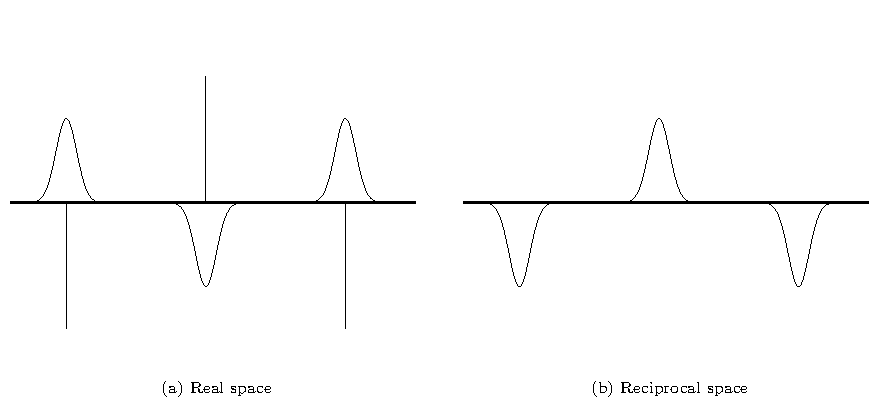
\includegraphics[width=0.8\textwidth]{./img/EwaldSum/EwaldSum}
	\caption{Schematic illustration of the \acs{ESM} charge distribution: in (a) point charges (represented by vertical lines) and the neutralizing Gaussian charge distribution; in (b) the counteracting Gaussian distribution.}
	\label{fig:ewald}
\end{figure}

The \ac{ESM} for electrostatic interaction works, as illustrated in figure~(\ref{fig:ewald}), considering each
point--like charge in the system surrounded by a neutralizing charge distribution of equal magnitude but opposite
sign that decays rapidly to zero. Simplifying the notation for a one dimensional system, the simplest functional
form is a Gaussian distribution centered in the position $r_i$ of the point--like charge $q_i$, of the form
\begin{equation}
	\rho_i(r) = \frac{q_i\alpha^3}{\pi^{3/2}}e^{-\alpha^2 (r - r_i)^2}
\end{equation}
that obeys the relation
\begin{equation*}
	\frac{q_i\alpha^3}{\pi^{3/2}}\int_{r_i-\epsilon}^{r_i+\epsilon}e^{-\alpha^2 (r - r_i)^2}\ dr \simeq q_i
\end{equation*}
where $(r_i-\epsilon; r_i+\epsilon)$ is a small interval around $r_i$. The energy contribution due to this set
up, the point--like charge \textit{and} the gaussian charge distribution, is given by
\begin{equation}
	U_r = \frac{1}{2}\sum_{i=1}^N\sum_{j=1}^N\ \sideset{}{'}\sum_{n_x,n_y,n_z}\ \frac{q_iq_j}{4 \pi \varepsilon_0} \frac{\erfc{(\alpha \| \vec r_i - \vec r_j + \vec n \|)}}{\| \vec r_i - \vec r_j + \vec n \|}
	\label{eq:ewaldReal}
\end{equation}
where the prime indicate that for $\vec n = 0$ must be $i\ne j$, $\erfc{(x)} = 1-\erf{(x)}$ is the complementary
error function and $\erf{(x)}$ is the error function. They are given by
\begin{equation}
	\erfc{(x)} = \frac{2}{\sqrt{\pi}}\int_{x}^{+\infty} e^{-t^2}\ dt, \qquad \erf{(x)} = \frac{2}{\sqrt{\pi}}\int_{0}^{x} e^{-t^2}\ dt
	\label{eq:erf}
\end{equation}

The point is that the summation involving the complementary error function in equation~\eqref{eq:ewaldReal} is
rapidly convergent and it needs very few terms so that a cut--off method can be safely used. The rate of
convergence depends on the $\alpha$ parameter: the bigger is $\alpha$, the more rapidly the series converges and
the shorter the cut--off radius can be. Thus the \ac{ESM} use the $\erfc{(r)}$ as $f(r)$ function in
equation~\eqref{eq:ewaldTrick}. Of course since we added a non physical neutralizing charge in the system, in
order to restore the real charge distribution, we must consider another distribution, called counteracting charge
distribution, of equal magnitude but opposite sign. Considering the identity in equation~\eqref{eq:ewaldTrick}
this lead to an energy contribution $U_f$ of the form $(1-f(r))/r$. But using the relation between \erfc{} and 
\erf{} functions, it becomes of the form $\erf{(r)}/r$. Another important trick is to compute $U_r$ in the 
\textit{real space} while $U_f$ in the \textit{reciprocal space}, thus considering its Fourier transform. This 
energy contribution is given by 
\begin{equation}
	U_f = \frac{1}{2}\sum_{i=1}^N\sum_{j=1}^N\ \sum_{k_x,k_y,k_z}\ \frac{1}{4\pi\varepsilon_0}\frac{4\pi}{L^3k^2}e^{-k^2/(4\alpha^2)}e^{\mathsf{i}{\vec k \cdot (\vec r_i - \vec r_j)}}
	\label{eq:ewaldReciprocal}
\end{equation}
where $\vec k = 2\pi\vec n/L$ are the reciprocal lattice vectors. Even $U_f$ converges rapidly as $U_r$ in
equation~\eqref{eq:ewaldReal}; then a cut--off method can be safely used. Nevertheless, opposite to $U_r$, the
smaller is $\alpha$, the shorter the cut--off can be. Clearly a proper \textit{balance} between the real and
reciprocal space summation is needed.

Since in equation~\eqref{eq:ewaldReal} even the self interaction with each Gaussian is included we need to add
another item for cancel it out; this is done by the self--term
\begin{equation}
	U_\text{self} = -\frac{\alpha}{\sqrt{\pi}}\sum_{i=1}^N\frac{q_i}{4\pi\varepsilon_0}
	\label{eq:EwaldselfTerm}
\end{equation}

Summarizing, the energy contribution of the electrostatic interactions by the \ac{ESM} is computed summing
equations~\eqref{eq:ewaldReal},\eqref{eq:ewaldReciprocal} and~\eqref{eq:EwaldselfTerm} to obtain
\begin{equation}
	\begin{aligned}
		U =&\quad\frac{1}{2}\sum_{i=1}^N\sum_{j=1}^N\ \sideset{}{'}\sum_{n_x,n_y,n_z}\ \frac{q_iq_j}{4 \pi \varepsilon_0} \frac{\erfc{(\alpha \| \vec r_i - \vec r_j + \vec n \|)}}{\| \vec r_i - \vec r_j + \vec n \|}\ + \\
		 &+ \frac{1}{2}\sum_{i=1}^N\sum_{j=1}^N\ \sum_{k_x,k_y,k_z}\  \frac{1}{4\pi\varepsilon_0}\frac{4\pi}{L^3k^2}e^{-k^2/(4\alpha^2)}e^{\mathsf{i}{\vec k \cdot (\vec r_i - \vec r_j)}}\ + \\
		 &- \frac{\alpha}{\sqrt{\pi}}\sum_{i=1}^N\frac{q_i}{4\pi\varepsilon_0}
	\end{aligned}
	\label{eq:EwaldEnergy}
\end{equation}
The first line is the real space contribution while the second is the Fourier energy contribution. Since the
self--interaction term is constant it does not affect forces computation. The \ac{ESM} offers a well defined
method to properly treat electrostatic interactions, nevertheless it is quite expensive in term of computational
resources. If $\alpha$ and the cut--off are constant, then the computation scales as $\sim N^2$.

For biomolecular applications most \ac{MD} tools set an equal cut-off radius for both Van der Waals interaction
and the real part of the Ewald summation~\eqref{eq:EwaldEnergy} in order to achieve for both a scaling of the
order $\sim N$. However in this way the computation of the reciprocal part in the Ewald
summation~\eqref{eq:EwaldEnergy} will be very inefficient as it scales as $\sim N^2$. In order to increase the
efficiency of the calculation of the Fourier transform various advanced methods can be used. They are all based
on the use of the \ac{FFT} method. In this way the reciprocal part can scale as $\sim N\ln N$. Since \ac{FFT}
requires discretized quantities, the idea of such methods, called \textit{particle mesh}, is to consider the
charge density spread on a mesh grid and then evaluate the electrostatic potential via solving the Poisson's
equation\footnote{Given a charge distribution $\rho(\vec r)$ then the associated electrostatic potential
$\phi(\vec r)$ can be calculated solving the Poisson's equation $\displaystyle \nabla^2\phi(\vec r) = -\frac{1}{\varepsilon_0} \rho(\vec r)$. If a charge $q$ is at position $\vec r$ its electrostatic potential energy is given by $U = q\phi(\vec r)$.}
using fast Poisson solver together with the \ac{FFT} method. This can be done, for example, exploiting the
\ac{PBC} in order to discretize and make periodic the Poisson's equation.
%\footnote{It is generally true that the Poisson's equation become ``easily'' solvable in Fourier space. Considering a one dimensional Poisson's equation, its Fourier transform is $k^2\varepsilon_0\tilde\phi(k) = \tilde \rho(k)$ where $\tilde\phi(k)$ and $\tilde\rho(k)$ are, respectively, the Fourier transform of the electrostatic potential and charge distribution.}.
Such algorithms include the \textit{particle--particle particle--mesh} method, \textit{particle mesh Ewald}
method, \textit{fast--Fourier Poisson} method and a recent methodology based on multi--scale mesh grid. The
efficiency and accuracy of such mesh--based algorithms depends strongly on the way in which the charges are
attributed to the mesh points, this makes the methods different. In the following we will describe the one used
in this thesis work, the \acf{PME} method.

\subsection{Particle mesh Ewald method}
The \acf{PME} method developed by Darden \etal\, \cite{DardenPME} is based on the \ac{ESM} so the starting point
is equation~\eqref{eq:EwaldEnergy}. As described above, the first part of the Ewald summation is computed in the
real space together with the Van der Waals contribution using the same cut--off radius. The reciprocal part
instead, is computed using \ac{FFT} method, in order to have a gain of performance. First, we need to
consider a grid mesh onto which the Gaussian counteracting charge distribution is spread. The basic idea, then,
is to calculate the electrostatic energy solving Poisson's equation through \ac{FFT} methods. The efficiency and
accuracy depend on the way the charges are distributed onto the grid. To do this a \textit{charge assignment
function}, $W(r)$ is introduced such that, considering for simplicity a one dimensional system, the fraction of a
charge at position $r$ assigned to a grid point at position $r_p$ is given by $W(r_p - r)$. Hence, if we have a
charge density $\rho(r)$ then the charges at the grid point $r_p$ are given by
\begin{equation}
	q_M(r_p) = \int_0^L\ W(r_p - r) \rho (r)\ dr
	\label{eq:meshAssign}
\end{equation}
where $L$ is the box length and, if $h$ is the grid spacing, $M = L/h$ is the number of mesh point. In
figure~(\ref{fig:gidAssign}) the charges assignment is schematically represented.

The assignment function should have the following proprieties: it should be an even function and it should be
normalized in such a way that the sum of the fractional charges equals the total charge of the system. Moreover
the best accuracy is obtained with a dense grid in order to reduce as much as possible the discretization of the
charge density. However the computational cost increases as the number of grid points: a balance between
efficiency and accuracy is clearly needed.
\begin{SCfigure}
	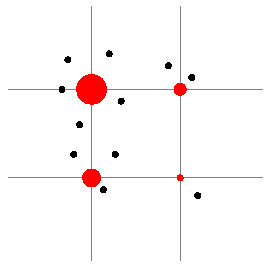
\includegraphics[width=0.35\textwidth]{./img/gridCharge/gridCharge}
	\caption{A schematic representation of the charge assignment. The black filled circles are a unit particle charge, while the red ones, are the charges assigned to grid points. The bigger is the circle, the more is the charge.}
	\label{fig:gidAssign}
\end{SCfigure}

A nice way to solve the problem of charge assignment is to shift the problem to the discretization of the Fourier
transform. This can be viewed as an interpolation problem. Consider the $e^{-\mathsf{i}\vec k\cdot \vec r_j}$
term in the Fourier transform of equation~\eqref{eq:ewaldReciprocal}. In general $\vec r_j$ does not correspond
to a mesh grid point, so this term is not part of a discrete Fourier transform. The idea, thus, is to interpolate
it in terms of the values of the complex exponential at the mesh points. Switching for simplicity to a one
dimensional system, if the mesh grid has $M = L/h$ points, a particle coordinate $r_j$ is located between mesh
points $[r_j/h]$ and $[r_j/h] + 1$ where $[\cdot]$ denotes the integer part; thus a $p$--order interpolation of
the exponential is of the form
\begin{equation*}
	e^{-\mathsf{i}kr_j} \simeq \sum_{i=1}^M W_{p}\left ( \frac{r_j}{h} - i \right ) e^{-\mathsf{i}khi}
\end{equation*}
where $W_{p}$ denotes the interpolation coefficient. A $p$--order interpolation means that only the $p$ mesh
points nearest to $r_j$ contribute to the sum. Assuming a point--like charge distribution the Fourier transform
of the charge density is therefore
\begin{equation*}
	\rho_k \simeq \sum_{i}e^{-\mathsf{i}khi} \sum_j\ q_iW_{p} \left ( \frac{r_j}{h} - i \right )
\end{equation*}
we can interpret the above expression as the discrete Fourier transform of the charge density
\begin{equation*}
	\rho(i) = \sum_j\ q_iW_{p} \left ( \frac{r_j}{h} - i \right )
\end{equation*}
but using equation~\eqref{eq:meshAssign}, it is nothing that the point--like charge distribution assigned to the
mesh point $i$ through the assignment function $W_{p}$.

We clearly see that the charge assignment problem is now shifted to the complex exponential interpolation. There
are two main methods to make the interpolation: the \textit{Lagrange interpolation method} and the \textit{Euler
SPLINE interpolation method}. The basic idea of the former is to use, as interpolating function, a polynomial
function of degree $ \le (n-1)$ where $n$ is the number of points to interpolate, that passes through all the $n$
points, and which is constructed with a summation over the \textit{Lagrange basis polynomials} as follow
\begin{equation*}
	P(x) = \sum_{i=1}^n y_i \prod_{\substack{k=1\\k\ne i}}^n \frac{x-x_k}{x_i - x_k}
\end{equation*}
where $(x_i;y_i)$ are the sets of points to interpolate. The main disadvantage of this method is that, even if
$P(x)$ is continuous everywhere, its derivative is not, thus it can lead to some instability in \ac{MD}
simulations.

The latter method, that is the most used in \ac{MD} tools, is based on the concept of \textit{SPLINE
interpolation}. Instead of using a unique interpolating function that passes through each point, the SPLINE
method uses a \textit{piecewise polynomial function}, called SPLINE, in which each piece is smoothly connected
and optimized to interpolate a subset of the points. The Euler SPLINE method use the \textit{exponential Euler
SPLINE} that is constructed with the basis of the Euler $n$--degree polynomials $A_n(x;\lambda)$ generated by the
following equation
\begin{equation*}
	\frac{\lambda - 1}{\lambda - e^z}e^{xz} = \sum_{n=0}^{+\infty} \frac{A_n(x;\lambda)}{n!}z^n
\end{equation*}
where $\lambda$ is a complex parameter and $z$ is a complex variable. The main properties of such SPLINE is that,
it is $n-1$ times analytic, continuously differentiable and then can solve the instability problem of the
Lagrange interpolation method. In literature the Euler SPLINE method is referred to as \textit{smooth} \ac{PME}
and the reader is addressed to the article by Essmann \etal\, \cite{EssmannSPME} for more technical details about
the interpolation procedure.

Summarizing, the \ac{PME} method is implemented with the following scheme
\begin{itemize}
	\item By the interpolation of the complex exponential in the Fourier transform of the Ewald summation, the
		  Gaussian counteracting charge distribution are spread onto the mesh grid;
	\item Poisson's equation for the discretized charges are solved through the \ac{FFT} methods;
	\item The $U_f$ energy contribution is obtained considering the inverse Fourier transform;
	\item Electrostatic forces are computed and assigned to the charged system particles.
\end{itemize}

The main advantages of the \ac{PME} algorithm are that the potential energy and forces are smooth functions of
the particles positions. The method offers a good energy conservation and offers a good balance between accuracy
and computational efficiency since it scales as $\sim N\ln N$. Moreover, despite we have described \ac{ESM} and
\ac{PME} applied to the electrostatic interaction, they can be used, with some changes, with all long--range
interactions and in general to all energy contributions that decay as $r^{-d}$, for example, even with the Van
der Waals energy contribution.

The general workflow shown in figure~(\ref{fig:MDscheme}) can be update adding the calculation of the bonded and the non--bonded interactions and the \ac{PME} contribution. In figure~(\ref{fig:PPCore}) a summary of the new workflow is shown.
\begin{figure}[ht!]
	\center
	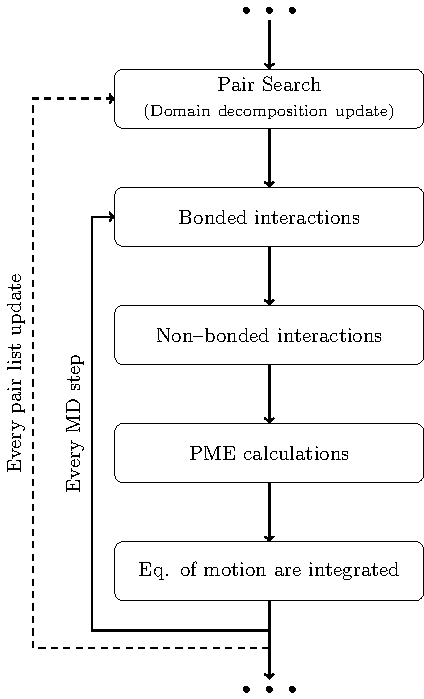
\includegraphics[width=0.5\textwidth]{./img/Schemi/PPCores}
	\caption{Schematic workflow of the particle interaction calculations inside an \acs{MD} simulation.}
	\label{fig:PPCore}
\end{figure}

\subsection{Charge representation}
\label{sec:chargeRep}
Even if some methods, such as the \ac{PME} one, have been developed to speed up the computation of electrostatic
energy contribution one of the main problems of \acp{FF} for biomolecular applications remains the \textit{charge
representation}: the way in which the charges of atoms or molecules are assigned to the system particles. The
problem arises from the necessity to represent the electron clouds and the interactions that generate.
Nevertheless this is crucial for a better description of most electrostatic phenomena such as polarizability of
molecules and polar solvent, solvation shell of charged ions, protein--ligand interactions, ion transport through
polar and non--polar medium, self assembly processes and so on.

The most common solution is the \textit{atom--centered ``partial charge'' approximation} in which the full charge
density of the molecule is replaced by fractional point--like charges assigned to each atom of the molecule.
Traditionally most non--polarizable \acp{FF} (as those we will use in this thesis work) assign to each atom of a
molecule a fixed partial--charge. The most used procedure for extracting partial--charges from molecular wave
functions is based on fitting atomic charges with the molecular electrostatic potential, computed with \textit{ab
initio} calculation such as \textit{density functional theory}. The fitting procedure consists in minimizing the
deviation between the electrostatic potential produced by the assigned charges and the molecular electrostatic
potential. Such representation is believed to be an important source of error in the electrostatics treatment.
Moreover with fixed charge assignment it is impossible to take into account those phenomena that involve a
transfer of charge inside the molecule, as polarization effect. The use of off--centered charges and/or higher
order atomic multipoles can significantly improve the treatment of electrostatics but of course it is necessary a
good balance between accuracy and performances since the electrostatic problem can rapidly drive to a loss of
computational efficiency.

\subsection{Polarization}
\label{sec:polarization}
Polarization refers to the redistribution of the electron charge density of a molecule in presence of an external
electric field, generated, for example, by charged ions or by another molecule. Polarization is responsible to
non--additive attractive inter-- or intra--molecular interactions which have many--body characteristics. These
effects have been recognized to have an important role in many biological interactions in which different
compounds are present. An increasing number of studies show that the lack of these effects can lead to serious
limitations, particularly, for systems that involve different environments such us water and proteins or water
and lipids. In \ac{MD} simulations polarization effects are included using either \textit{implicit} or
\textit{explicit} methods.

The implicit method completely avoids the many--body calculations by including a mean polarization effect in the
functional form of the interaction potential. The general idea is to surround all the simulation box by a
transparent medium with a relative dielectric constant $\varepsilon_r$. In this way the polarization effect is
taken into account considering a mean field theory and solving the Poisson's equation to determine the
electrostatic potential due to system charges by the substitution
$\varepsilon_0\rightarrow\varepsilon_0\varepsilon_r$. Since it avoids many--body calculations, this method gives
an incomparable gain in performances but it must be carefully used. The main disadvantage is that the mean
polarization effect is added to all system particles and this wash out all the details about a possible
polarization effect in a molecule. Moreover the electrostatic interaction between charged particles is affected
by the mean field effect. This produce a correct electrostatic interaction for particles inside the same solvent
for which the implicit medium is parameterized. Otherwise, if the simulation box is composed by different
chemical environments such as a polar and non--polar compounds, using the same dielectric constant would lead to
badly calculate the electrostatic interactions for particles in the non--polar environment. Thus, this method can
be safely used when our system is composed principally by one kind of solvent, for example water.

The way to correct the above behavior is to use an explicit method. As the name suggests, the polarization effect
is taken into account for every molecule in the system by an its proper model included in the \ac{FF}. The
general idea is to add some more internal \ac{DOF} to a molecule or atom to take into account the movement of
charges and/or split the point--like charge assigned, for example, to a chemical group, to a partial-charge
assigned to each particles of the chemical group itself. This can be done for every molecule or atom in the
system and thus it is the optimum to better describe systems with different chemical environments. Obviously this
method is more time consuming compared to the first.

%\subsection{Atomistic model}
\section{Coarse--Grained model}
\label{sec:CGModel}
As we have introduced at the beginning of this section, for biomolecular applications two main classes of
classical \acp{FF} exist: atomistic \acp{FF} and \ac{CG} \acp{FF}. Since the atomistic model takes into account
all the atoms in a molecule it is obviously the most realist and accurate \ac{FF}. Nevertheless the large number
of \ac{DOF} of atomistic \acp{FF} leads to a loss of computational performance. Moreover, basically, the
atomistic \acp{FF} are efficient until the physical proprieties can be properly sampled on a time scale of 
hundred of nanoseconds over a length scale of a few nanometers. As the time and length scales increase more and 
more time is needed to carry out a complete simulation. Unfortunately many biological processes involving lipid 
membranes and other organic molecules, including synthetic compounds, take place on much longer time (of the 
order of microseconds nor milliseconds) and length scales (of the order of tens nanometers).

One possible solution is to \textit{integrate out} some \ac{DOF}, preserving those that are relevant for the
problem in exam: this procedure is called \textit{coarse--graining}. The basic units of \ac{CG} \acp{FF} are
called \textit{beads}, each representing a group of atoms or a well defined chemical moiety. The size of the
group of atoms that is represented by a single bead determines the degree of coarsening of the \ac{FF}. Even in
this case, all the general features described above, apply: functional forms need to be chosen and their
parameterization need to be adjusted so as to reproduce the desired target properties. In figure~(\ref{fig:CGLevels}) different levels of coarse--graining are showed.
\begin{figure}[h!t]
	\centering
	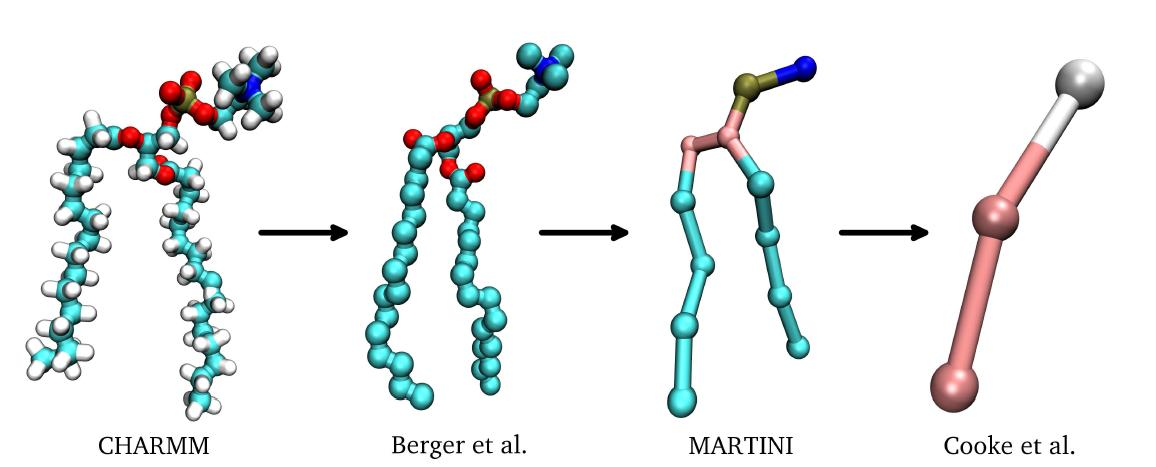
\includegraphics[width=0.7\textwidth]{./img/CGMapping}
	\caption{Different levels of the coarse--graining of a phospholipid. From left to right increasing levels of coarse--graining. Taken from \cite{CoarseGrainingMapping}.}
	\label{fig:CGLevels}
\end{figure}

The first step in the development of a \ac{CG} model is the \textit{mapping} procedure. This establishes a link
between the atomistic model and the \ac{CG} one. There is not a unique or correct procedure to perform the
mapping because it depends on the desired coarse--graining level, on the time and length scales that one wants to
correctly sample and on the properties one wants to reproduce. For biological applications \ac{CG} \acp{FF} are
often designed to reproduce specific thermodynamic properties such as surface tension, free energy of
partitioning, free energy of hydration and so on. \ac{CG} \acp{FF} employed in the material sciences (e.g.
polymer science) often use as a target the material structural properties.

In general a \ac{CG} \ac{FF} is more computationally efficient than an atomistic one for the following reasons
\begin{itemize}
\item the \ac{DOF} of the system are reduced due to the \ac{CG} procedure with the consequence that a smaller number of interactions and forces has to be computed;
\item bead--bead interactions, which result from the removal of finer structural details, are softer than atom--atom interactions;
\item vibrational modes are slower, and their sampling can be achieved using larger \ac{MD} time steps than in atomistic simulations;
\item softer interactions imply a smoother \ac{PEF} which leads to faster diffusion.
\end{itemize}

\section{MARTINI: a Coarse--Grained Force--Field}
\label{sec:martini}
\martini is a \ac{CG} \ac{FF} developed by Marrink \etal\, \cite{Martini} for organic solvents and lipids and
then extended to proteins \cite{MartiniProtein}, carbohydrates \cite{MartiniCarbo} and a broad class of polymers
\cite{MartiniPolymers}. \martini is based on a chemical building block approach. Such \martini blocks or beads
represent small chemical moieties and they are extensively calibrated in order to construct a large variety of
organic molecules. As we shall see in section~\ref{sec:martiniParam}, the \ac{FF} is based on accurately
reproducing the interaction between polar and non--polar chemical compounds. The main target property is intact
the \textit{partitioning free energy} between water and a large number of organic solvents, i.e. the free energy
of transfer of chemical moieties from polar and non--polar solvents.

\subsection{Mapping}
The mapping of the \martini beads is based on a four--to--one scheme that groups four heavy atoms like C, S, O
and so on, plus their associated hydrogen atoms, into a single interaction site. Consistently four water
molecules are modeled with one \martini bead. An example of the mapping procedure including both atomistic and
\ac{CG} descriptions is shown in figure~(\ref{fig:martiniMapping}).
\begin{figure}[!ht]
	\centering
	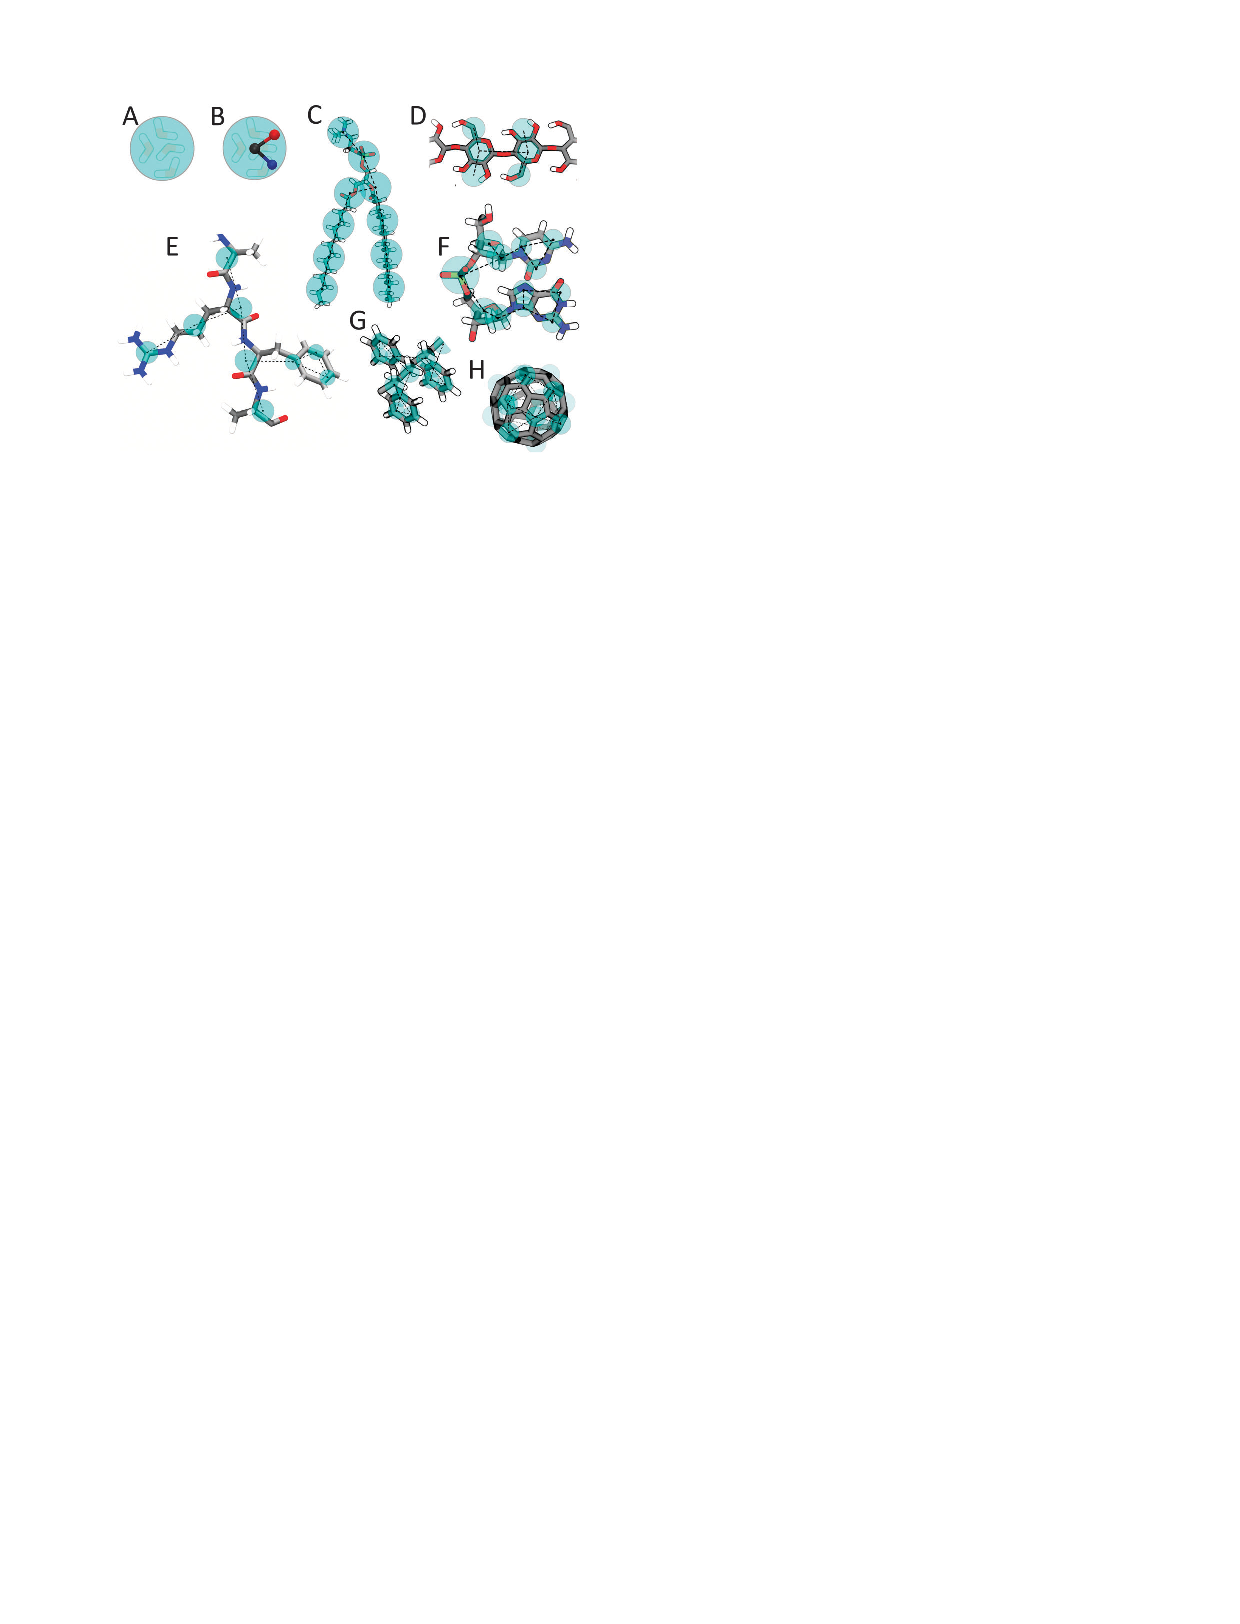
\includegraphics[width=0.5\textwidth]{img/martiniMapping}
	\caption{\martini mapping and atomistic structures compares of some molecules: (A) Standard water bead, (B) polarizable water bead, (C) \acs{DMPC} lipid, (D) Polysaccharide fragment, (E) Peptide, (F) DNA fragment, (G) Polystyrene fragment and (H) Fullerene molecule. In all cases \martini \acs{CG} beads are shown as cyan transparent beads overlaying the atomistic structure. Taken from \cite{MartiniReview}.}
	\label{fig:martiniMapping}
\end{figure}

There are four main bead types: polar (P), non--polar (N), apolar (A) and charged (Q). Each bead type has a
number of subtypes to take into account a more accurate representation of the chemical nature of the moieties due
to the underlying specific atomistic structure. These subtypes are distinguished by the hydrogen bonding
capabilities: donor (d), acceptor (a), both donor and acceptor (da) and none ($0$) and/or by their degree of
polarity: lowest polarity ($1$), $\dots$, highest polarity ($5$).

\begin{SCtable}\footnotesize
	\begin{tabular}{lc}
		\toprule
		Level  & $\epsilon$\,[kJ/mol] \\ \midrule
		O	   & $5.6$	 \\ \midrule
		I      & $5.0$	 \\ \midrule
		II	   & $4.5$	 \\ \midrule
		III	   & $4.0$	 \\ \midrule
		IV	   & $3.5$	 \\ \midrule
		V	   & $3.1$	 \\ \midrule
		VI	   & $2.7$	 \\ \midrule
		VII	   & $2.3$	 \\ \midrule
		VIII   & $2.0$	 \\ \midrule
		IX     & $2.0$	 \\ \bottomrule
	\end{tabular}
	\caption{Interaction strength parameter ($\epsilon$). The last one is for the special case $\sigma=0.62$~nm.}
	\label{tab:martiniEpsilon}
\end{SCtable}

\subsection{Interactions potential}
\label{sec:martiniPotential}
\paragraph{\textbf{van der waals interactions}} The functional form describing pairwise Van der Waals interaction
is a Lennard--Jones $12-6$ potential as in equation~\eqref{eq:lj126}. For most beads the $\sigma$ parameter is
set equal to $0.47~$nm except for the Q--C$_1$ and Q--C$_2$ interactions for which $\sigma = 0.62$~nm. This is
consistent with reproducing the hydration shell when a charged bead (Q) is dragged into an apolar medium. The
strength of the interactions is instead dived into ten levels, reported in table~(\ref{tab:martiniEpsilon}). The
association of the interaction strength with each \martini beads is shown in
figure~(\ref{fig:martiniInteractions}).
\begin{figure}[h!t]%
	\center
	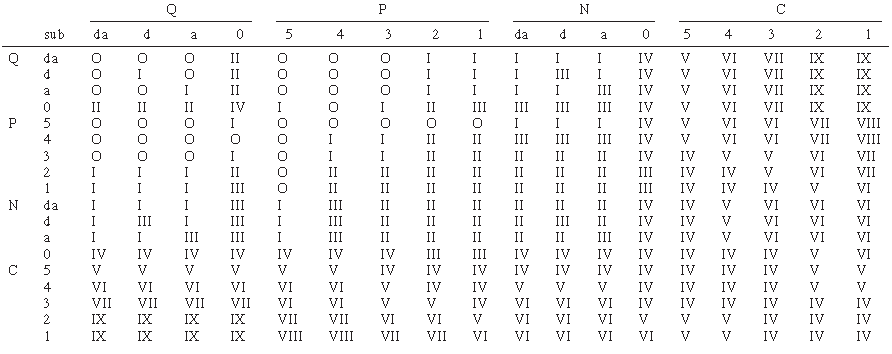
\includegraphics[width=\textwidth]{img/martiniInteractions.pdf}%
	\caption{Interaction strength association matrix for the \martini bead types and subtypes. Taken from \cite{Martini}.}
	\label{fig:martiniInteractions}
\end{figure}

\paragraph{\textbf{electrostatic interactions}} Electrostatic charges are assigned using the atom--centered
approximation, as described in~\ref{sec:chargeRep}. The charges of the \martini beads are empirically assigned at
the center of the beads and correspond to the net charge of the chemical moiety they represent. Water, for
example, is described by a neutral P$_4$ beads. Van der Waals interactions are responsible for take into account,
effectively, the effects of polarizability together with the use of an implicit medium with a dielectric constant
$\varepsilon_r = 15$. However, as we shall see in section~\ref{sec:pw}, to avoid the problems with the implicit
medium described in~\ref{sec:polarization}, especially for lipid membranes for which the dielectric constant in
the hydrophobic region is much smaller, Yesylevskyy \etal\, \cite{PW} have developed a more sophisticated \ac{CG}
water model, called \ac{PW}, to take into account a better water behavior.

\paragraph{\textbf{bonded interactions}} They include only bond length and an angle harmonic contributions. The
former is modeled with a harmonic potential as the first term in equation~\eqref{eq:bondPEF}, with the same bond
constant for all bead types: $k^b = 1250$~kJ/(mol\ nm$^2$) and an equilibrium distance of $l_0 = 0.47$~nm. The
latter is modeled as a cosine--type harmonic potential
\begin{equation}
	U = \frac{1}{2}k^a (\cos(\theta) - \cos(\theta_0))^2
	\label{eq:martiniAngle}
\end{equation}
whose parameters are: $k^a = 25$~kJ/mol and $\theta_0 = 180^\circ$ for aliphatic chains; $k^a = 45$~kJ/mol and
$\theta_0 = 120^\circ$ for \texttt{cis} double bonds and $k^a = 45$~kJ/mol and $\theta_0 = 180^\circ$ for
\texttt{trans} unsaturated bonds. Moreover, especially for ring systems, an improper dihedral angle harmonic
potential can be used to prevent out of plane distortion. The form is
\begin{equation*}
	U = k_{id} (\theta_{ijkl} - \theta_0)^2
\end{equation*}
where $\theta_{ijkl}$ denotes the angle between the planes described by atoms $i,j,k$ and $j,k,l$; $k_{id}$ and
$\theta_0$ are, as usual, the force constant and equilibrium angle.

\subsection{Simulation parameters}
The \martini \ac{FF} was originally developed using a shifted cut--off scheme for both Lennard--Jones and
electrostatic potentials with a cut--off radius $r_c = 1.2$~nm. The Lennard--Jones potential was shifted from
$r_s = 0.9$~nm to $r_c$ while from $r_s = 0.0$~nm to $r_c$ for the electrostatic potential. The neighbor list is
constructed as described in the first part of~\ref{sec:neighbor} with a refresh rate of $10$ \ac{MD} steps.
Recently the more efficient Verlet cut--off scheme was tested by Marrink \etal\, \cite{MartiniReview} and used
with the \martini \ac{FF} with a cut--off radius of $r_c = 1.1$~nm, a Verlet buffer tolerance of $0.005$~kJ/(mol\
ps) and a minimum refresh rate of $10$ \ac{MD} steps (often, depending on the hardware, it can be dynamically
increased to $30$ or $40$ \ac{MD} steps getting better performances).  Moreover, the treatment of the
electrostatic interaction can be safely updated to the \ac{PME} method together with the Verlet cut--off scheme.
This new set--up was largely tested by Yesylevskyy \etal\, \cite{PW}. In this case the cut--off radius was set to
$r_c = 1.2$~nm with the same Verlet buffer tolerance; the \ac{PME} grid spacing was set to have a lower bound of
$0.12$~nm and the interpolation was set to a fourth-order. Moreover, with the use of \ac{PW}, as we shall see,
the dielectric constant should be reduced to $\varepsilon_r = 2.5$. In all cases a time step
$20\le\delta t\le 40$ is suitable for a great number of applications. It should be clear that changing these
simulation parameters must be followed by a retest of the main properties of the \martini \ac{FF}.

\subsection{Parametrization}
\label{sec:martiniParam}
In order to parametrize the \martini \ac{CG} \ac{FF} a set of thermodynamics properties, obtained from \ac{MD}
simulations, are compared and fitted against those experimentally measured. These properties are the \textit{free
energies of vaporization}, \textit{hydration} and \textit{partitioning} between water and a set of organic
compounds such as hexadecane (H), chloroform (C), ether (E) and octanol (O). The free energy of hydration was
obtained from the partitioning of \ac{CG} beads between bulk water in equilibrium with its vapor. Similarly the
free energy of vaporization was obtained considering a simulation box with the selected \ac{CG} bead in a liquid
phase in equilibrium with its vapor. From the equilibrium densities of the particles in both phases the related
free energies can be computed from
\begin{equation*}
	\Delta G = k_B T\ln \left ( \frac{\rho_{\text{vap}}}{\rho_{\text{bulk}}} \right )
\end{equation*}
All the simulations were performed in a canonical $NVT$ ensemble.

The partitioning free energy between water and an organic solvent was obtained in a $NPT$ ensemble, considering a
simulation box half filled of water and half of the organic solvent. Then a small fraction of the \ac{CG}
particle for which the partitioning free energy is to be computed, was placed in the simulation box. From the
equilibrium densities of the particles in water $\rho_{\text{wat}}$ and in organic solvent $\rho_{\text{oil}}$,
the free energy of transfer can be computed from
\begin{equation*}
	\Delta G_{SW}^{\text{part}} = k_B T \ln \left ( \frac{\rho_{\text{oil}}}{\rho_{\text{wat}}}\right )
\end{equation*}
where $S$ indicate the organic solvent.

In figure~(\ref{fig:martiniTarget}) a summary of the results is reported. As one can see the model has bad
performances for what concerns the free energies of vaporization and hydration, which are too high with respect
to experimental data. Instead, the partitioning free energies match very well. Thus the model is not very
accurate for vapor--liquid systems but it is reliable at describing the behavior of liquid phases with
different degrees of hydrophobicity.
\begin{figure}[h!t]%
	\center
	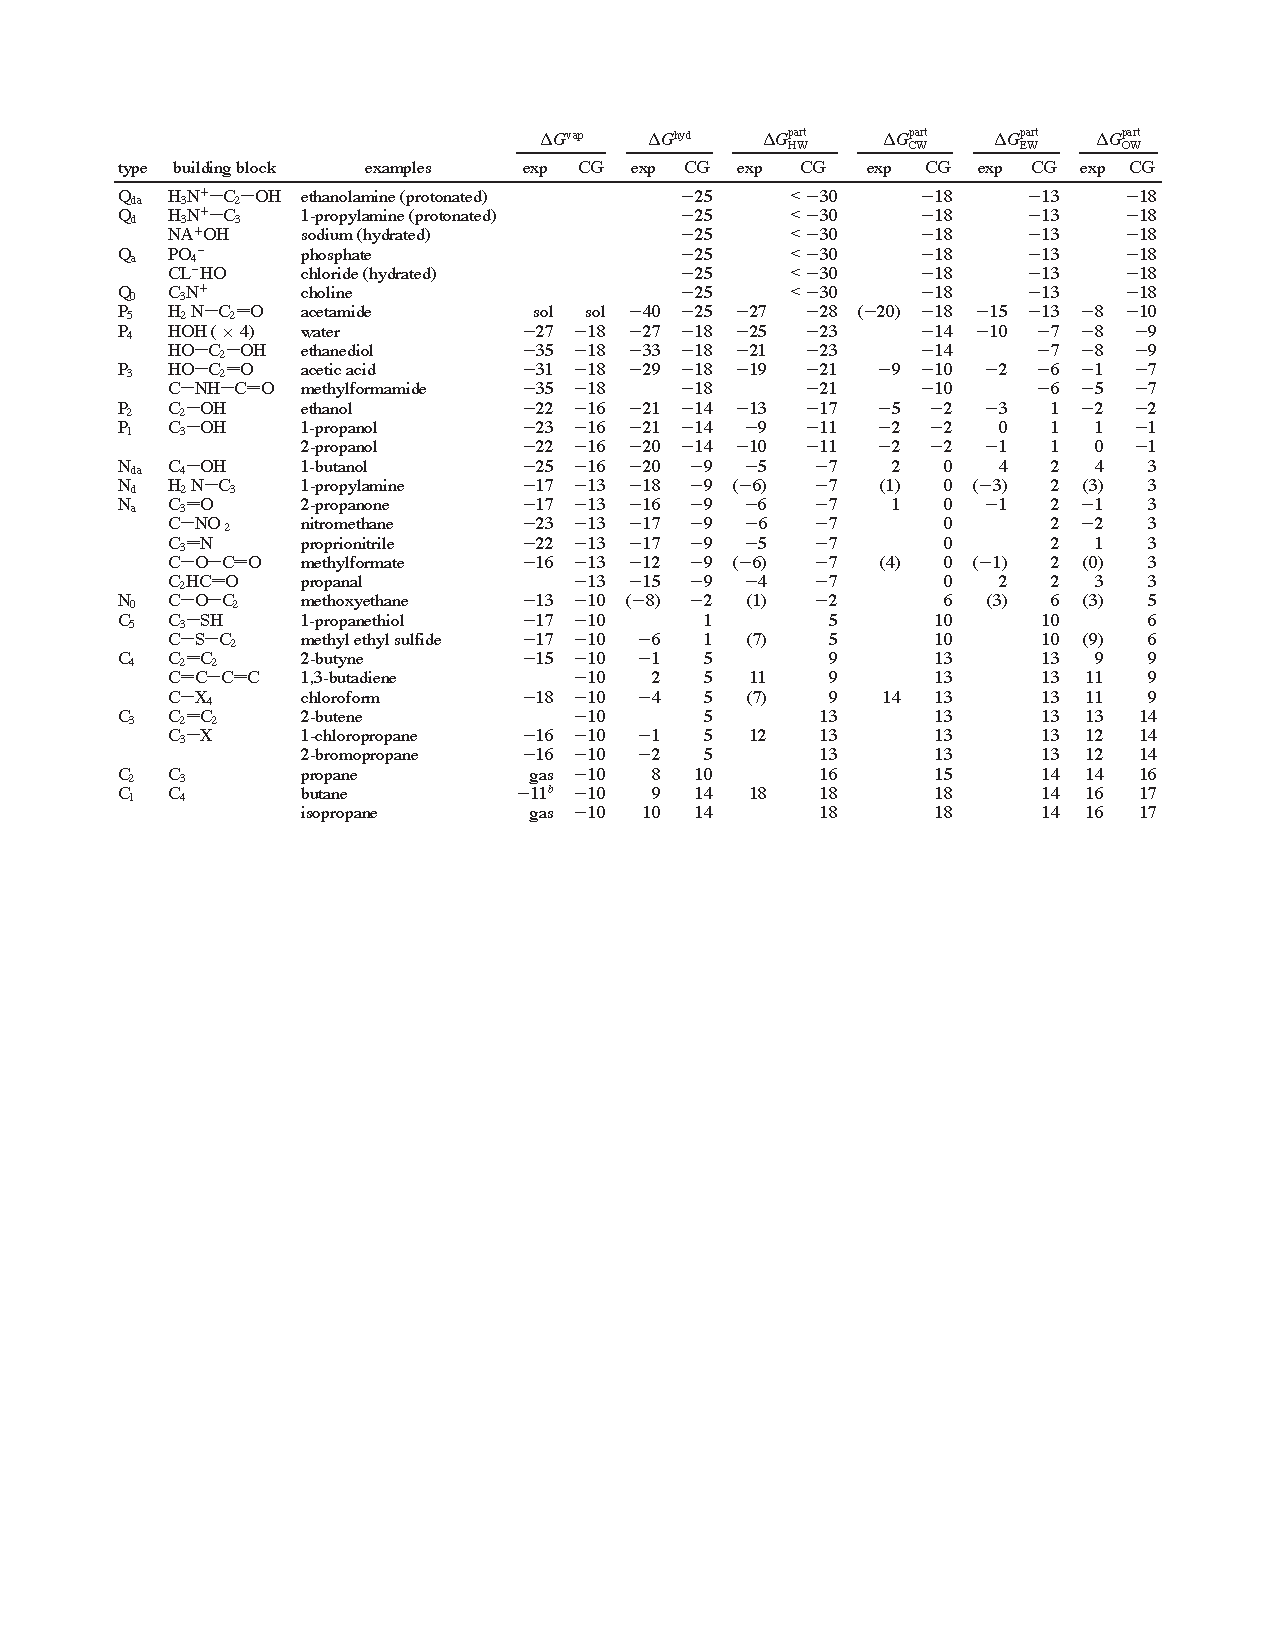
\includegraphics[width=\textwidth]{img/martiniTarget}%
	\caption{Results summary: free energies of vaporization $\Delta G^\text{vap}$, hydration $\Delta G^\text{hydr}$ and partitioning $\Delta G^\text{part}$ between water (W) and organic solvents (hexadecane (H), chloroform (C), ether (E) and octanol(O)) compared to experimental values. Experimental properties in parentheses are estimates obtained from comparison to similar compounds. The statistical accuracy of the free energies obtained from the simulations is $\pm 1$~kJ/mol. $^b$ The temperature for the experimental data is $273$~K. Taken from \cite{Martini}.}
	\label{fig:martiniTarget}
\end{figure}

\subsection{Polarizable Water model}
\label{sec:pw}
Water plays a crucial role in any biomolecular system. It is important thus to correctly describe its behavior.
Since the \martini water model does not directly take into account the electrostatic interaction between water
and water and other environment because it does not have any charge and it interact only via Van der Waals
interaction, a simple implicit medium is used to take into account the main electrostatic effects of water,
screening and polarizability. In reality, however, any biomolecular process involves charged species moving
between regions of different dielectric constant. Due to the change in electrostatic screening between those
environments, the strength of the interaction between the moving charges and the surrounding molecules also
changes. This effect can not be taken into account by implicit medium models. In order to capture the
inhomogeneous nature of the dielectric response an explicit medium has to be used.
\begin{figure}[!ht]
	\centering
	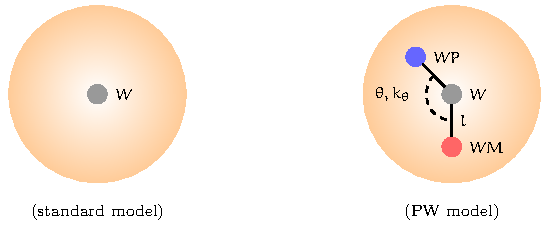
\includegraphics[width=0.7\textwidth]{./img/PWModel/PWModel}
	\caption{Schematic representation of the \acs{PW} bead. Shaded orange spheres correspond to the Van der Walls radii of the central neutral particle $W$. The blue particle is the positively charged while the red is the negatively charged.}
	\label{fig:PW}
\end{figure}

In the same fashion of the \martini philosophy, Yesylevskyy \etal\, \cite{PW} have developed a \acf{PW} model
that better describes the real behavior of water. As before one \ac{PW} bead is associated to four water
molecules. The new water bead consists of three particles instead of one in the standard \martini model. In
figure~(\ref{fig:PW}) the topology of the \ac{PW} and a comparison with the old model is shown. The central
particle $W$ is neutral and interacts with other particles in the system with the only Lennard--Jones potential.
There are two additional particles, namely $WP$ and $WM$, that are bound to the central particle and carry a
positive and negative charge $|q| = 0.46\mathsf{e}$ respectively, where
$\mathsf{e} = 1.60217653(14) \cdot 10^{-19}$~C is the unit electron charge. They interact with other particles in
the system by the Coulomb interaction only. The bonds $W-WP$ and $W-WM$ are constrained to have a fixed distance
$l = 0.14$~nm. The electrostatic interaction between $WP$ and $WM$ inside the same bead are exclude, thus they
are invisible to each other and they can rotate around the $W$ particle. As a consequence the dipole momentum of
the water bead depends on the relative angular position $\theta$ of $WP$ and $WM$: it can vary from zero
($\theta = 0$) to $2ql$ ($\theta = \pi$). A harmonic angle potential with equilibrium angle fixed to
$\theta_0 = 0$ and a force constant $k_\theta = 4.2$~kJ/(mol\ rad$^2$) is added to control the rotation of
$WP$ and $WM$ particles around the $W$ particle, so to adjust the distribution of the dipole momentum. The value
of the equilibrium angle is consistent with the fact that in an apolar medium the total dipole momentum of a
water molecule is zero.

Since in this model the screening and polarization effects are treated explicitly the global dielectric constant
is then reduced from $\varepsilon_r = 15$, used in the standard \martini, to $\varepsilon_r = 2.5$. Moreover,
since the \ac{PW} beads attract each other stronger then the standard water beads (P$_4$ type), because of the additional electrostatic interactions, the strength $\epsilon_{WW}$ of the Lennard--Jones interaction between $W$ particles must be reduced. Water properties, especially the hydration free energy compared to the standard water model, and the lipid membrane behavior are reproduced satisfactory if the Lennard--Jones strength is changed from a
$I$ level (see table~(\ref{tab:martiniEpsilon})) to a $95\% $ of it. Since even in this case the hydration free energy was too high, the same apply to the cross interaction terms between $W$ particle and the other \martini beads. Instead, $\sigma$ remains unchanged to $0.47$~nm. In addition to this, in order to recover the correct partitioning behavior, the self terms between Q type beads are generally decreased; while the cross terms are generally increased. In figure~(\ref{fig:PWMartini}) a summary of the new interaction terms between Q type beads and the other beads is shown.
\begin{figure}[!ht]
	\centering
	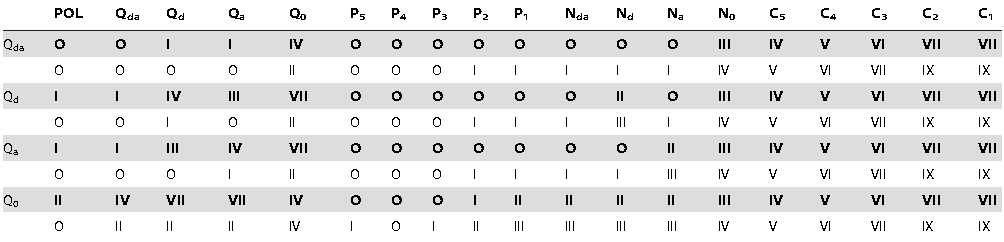
\includegraphics[width=\textwidth]{./img/PWMartini}
	\caption{New interaction strength between Q type beads and the other beads. New values in bold font, old values in normal font. See table~(\ref{tab:martiniEpsilon}) for the interaction levels. POL is the name of the \martini bead type associated to particle $W$ inside a $PW$ bead. Taken from \cite{PW}.}
	\label{fig:PWMartini}
\end{figure}

The parametrization of $q$, $k_\theta$ and $\epsilon_{WW}$ are obtained, in addition to the basic target
properties of the \martini \ac{FF}, also trying to reproduce the dielectric constant $\varepsilon_{W}$, density
$\rho$ and dipole momentum of a pure water phase. The above parameters of the \ac{PW} model are summarized in
table~(\ref{tab:PWParam}) while a comparison of the results obtained with the \ac{PW}, the standard \martini
water and the experimental data are summarized in table~(\ref{tab:PWRes}). For more details about the
parameterizations and testing methods the reader is
addressed to the article by Yesylevskyy \etal\,\cite{PW}.

Moreover, the authors found that, in addition to the \ac{PW} model, the use of \ac{PME} method contributes to a
more realistic description of the processes involved in biomolecular environments. In particular, some
interesting results of utility for this thesis work concern a better description of the properties of lipid
membranes, as we shall see in chapter~\ref{chap:membraneNP}.

\begin{SCtable}
	\centering
	\begin{tabular}{ll}
		\toprule
		$|q| = 0.46\mathsf{e}$				\\ \midrule
		$l = 0.14$~nm						\\ \midrule
		$\theta_0 = 0$						\\ \midrule
		$k_\theta = 4.2$~kJ/(mol\ rad$^2$)	\\ \midrule
		$\epsilon_{WW} = 4$~kJ/mol			\\ \midrule
		$\sigma = 0.47$~nm					\\ \bottomrule
	\end{tabular}
	\caption{Summary of the parameters used in the \acs{PW} model. See \cite{PW} for details.}
	\label{tab:PWParam}
\end{SCtable}

\begin{table}
	\centering
	\begin{tabular}{lrrr}
		\toprule
		\,	& \acs{PW} &  \martini water & Experimental \\ \toprule
		$\rho$~[kg/m$^3$]				& $1043$  & $1013$  & $997$		\\ \midrule
		$\overline{p}$~[D] 				& $4.9$   & $-$ 	& $4.4^a$		\\ \midrule
		$\varepsilon_{W}$ 				& $75.6$  & $-$ 	& $78.4$	\\ \midrule
		$T_\text{melt}$~[K] 			& $282$   & $290$ 	& $273$		\\ \midrule
		$\Delta G^\text{hyd}$~[kJ/mol] 	& $-18.7$ &	$-18$	& $-27$		\\ \midrule%\subsection{Applications}
		$D_{WW}~[10^{-5}$~cm$^2$/s]		& $2.5$   & $2.0$   & $2.3$		\\ \bottomrule
	\end{tabular}
	\caption{Summary of the results obtained with the \acs{PW}, standard \martini water and the experimental data at $T=300$~K. $\overline{p}$ is the average dipole momentum of a pure water box and $D_{WW}$ is the self--diffusion coefficient. \footnotesize $^a$ In order for a comparison to be made, this data is obtained from an atomistic simulation of $1600$ SPC/E water molecules and the average dipole momentum $\overline{p}$ is obtained averaging over a groups of four molecules, randomly chosen; see \cite{PW} for more details.}
	\label{tab:PWRes}
\end{table}

%One is the translocation of charged ions through a lipid bilayer that is described in a more realistic detail: the authors found that the simulations with \ac{PW} and \ac{PME} are approaching the atomistic results better then the standard \martini \ac{FF}. Another important phenomenon about lipid membranes consist in the electroporation of membrane by \ac{PW} beads due to an electric field across the membrane (for example, created by a cross membrane ions imbalance) and, related to this, the translocation of ions across the membrane helped by a so called ``\textit{water finger}'' a water defect inside the membrane that seems to be the trigger of the ions translocation. Such phenomenons are clearly evident in atomistic simulations however never occurred using the standard \martini \ac{FF} thus the importance to use the \ac{PW} model together with \ac{PME} method.

\subsection{Limitations of MARTINI FF}
As we have seen in~\ref{sec:CGModel} the \ac{CG} \acp{FF} are computationally advantageous, still a price has to
be paid. Although the \martini \ac{FF} is still a fine \ac{CG} \ac{FF}, some limitations are shared with other
\ac{CG} models at a fundamental level, such as the chemical and spatial resolution, which are both limited
compared to atomistic models. An important issue is the underestimation of the entropy which respect to the
atomistic case, that is a consequence of the \ac{DOF} reduction process. Since in the \martini \ac{FF} the
partitioning free energy $\Delta G = \Delta H - T\Delta S$ must be consistent which the experimental data, the
intrinsic loss of entropy imply a reduction of the enthalpy contribution, generating an imbalance between them.
If a $NVT$ ensemble is used the correct potential is the Helmholtz free energy $\Delta A = \Delta U - T\Delta S$,
thus the imbalance is between the internal energy and the entropy. This means that the use of a \ac{CG} model
with a $NVE$ ensemble leads to a problem of energy conservation. Anyway this is not our case since we only use a
$NVT$ or a $NPT$ ensemble with an external thermostat coupling.

Another consequence of the use of a \ac{CG} \acp{FF} is related to the \ac{FES} that becomes smoother respect to
the atomistic case. This effectively results in more sampling of the energy landscape in a given time period,
speeding up the dynamics of the system. Moreover even the \ac{PEF} becomes smoother, in particular the bonded
contributions, allowing the use of an higher time steps with longer simulation times. However the speed--up is
not easily predictable and is not likely to be the same for different systems and maybe it is dependent on the
type of molecule. Nevertheless for the \martini \ac{FF} an average scaling factor of four, based on lateral
diffusion coefficients of lipids in membranes, is commonly used, of course with some care. Another smaller source
of errors is due to the choice of masses: since ensemble properties are not affected by particle masses, in order
to increase the efficiency, all the \martini beads have the same mass of $72$~amu. This leads in some uncertainty
in the dynamics of the system making the time scaling for different beads non--trivial.

A problem involving the Lennard--Jones potential as a model of Van der Waals interactions in \martini, is that
the steep repulsion leads to an over--structuring of fluids compared to atomistic models. As we can see from
table~(\ref{tab:PWRes}) the direct and most evident implication is the melting point of the standard \martini
water that is $290 \pm 5$~K. A practical partial solution is the use of the so called ``anti--freeze'' particles
named BP$_4$ type. The Lennard--Jones interaction between these particles and water is modified with a slightly
larger Van der Waals radius parameter, $\sigma = 0.57$~nm and a stronger interaction to be a level $O$ (see
table~(\ref{tab:martiniEpsilon}) for the interaction level). Marrink \etal\, suggest that a mole fraction of
$n_{\text{af}} = 0.1$ is sufficient to prevent freezing without affecting the other properties of water.
%Some other properties of water are not accurate described such us the surface tension of air/water interface that leads in problem to water/oil interfaces formation.
Using the \ac{PW} model these properties improve slightly, see table~(\ref{tab:PWRes}). For a more comprehensive
discussion about the limitations of the \martini \ac{FF} the reader is addressed to the review by Marrink \etal\, \cite{MartiniReview}.

